%% This is a dissertation template for use with Masters/PhD dissertations at the University of Arizona.
%%
%% This template was created in 2022 and subsequently updated by Samuel A. Myers to greatly simplify the 
%% old thesis template. This was done to make the template easier to use, less intimidating, and because
%% the old template had not been actively updated in over a decade. Furthermore, in recent years the Grad 
%% College has greatly relaxed thesis requirmenets, and so the hyperspecific formatting guidelines utilized in
%% the old template were no longer relevant. 
%%
%% Also note that all of the AAS compatability has been explicitly removed, however it can easily be added back
%% by simply including the relevant packages in the preamble. This shouldn't break the template (with the exeption
%% of deluxetable, which is evil and should never be used).
%%
%% This template was made to match the guidelines as listed here (https://arizona.app.box.com/v/grad-gsas-dissformat)
%% in Jan of 2024. As always, check to make sure that your thesis is compliant before submitting it. If you
%% find any errors, please let the current LPL template manager or grad webmaster know. Furthermore, Be aware that 
%% there are some "secret" requirements that they don't tell you about until you are submitting your thesis. For
%% the most part these should be small things, but if you have problems, reach out to the template manager.
%%
%% This template is based on an old template that utilized a custom LaTeX class. That template was
%% worked on from the late 80's to early 2000's by a series of graduate students in the Department of
%% Planetary Sciences. Although much of that template has been scrapped, this template is still heavily based
%% on it, and much of their sample text has been utilized. The following is a list of all the students who
%% have worked on various thesis templates.
%%
%% Peter Halverson	1989 (non-LPL)
%% William D. Sears	1994
%% Rov Vervack		1996
%% Andrew Rivkin	1997
%% Joe Spitale		2001
%% Dave O'Brien		2003
%% Ross A. Beyer	2004
%% Jim Richardson	2005
%% Terry Hurford	2005
%% Curtis S. Cooper	2007
%% David A. Minton  2009
%% Samuel A. Myers	2024
%%
%% To compile this template, the recommend run sequence is:
%% PdfLaTeX + Bib(la)tex + PdfLaTeX (x2)
%% This should ensure the references, figures, tables, table of contents, etc are all updated fully and correctly.
%% If using Overleaf, Overleaf should take care of this automatically.
%%
%% If you have any questions and its before ~2026, please feel free to email sammyers@arizona.edu


\documentclass[12pt]{report} %Sets default font size and report format
    %To align the page numbers for double sided printing use \textbf{\documentclass[12pt,twoside]{report}}
    %You will also have to change a line (noted below) under Set up for fancyhdr and comment out a line
    %under both the List of Figures and List of Tables (also noted below).
    %Note that twosided page numbers are nicer for printing, but ARE NOT COMPLIANT with the requirements

%------------------------------------Import our packages----------------------------------------------
%These are all the packages required for the base template. Note that you may find other packages useful
%to deal with the particular needs for your dissertation.

\usepackage[margin=1in]{geometry}	
	%Sets 1in margin on all sides. Required for ProQuest/UMI. Note there are otherwise no margin
	%formatting requirements from the college.
\usepackage{amsfonts,amsmath,amssymb,wasysym}	
	%Includes basic math symbols, including astronomy symbols. Note some symbols may require being
	%placed in their own brakcets to work properly, ie {\odot}
\usepackage{fancyhdr} 							
	%Provides more customization of the headers
\usepackage[explicit]{titlesec}	
	%Allows for cusotmization of section heading appearances						
\usepackage{indentfirst}						
	%By default indents the first line of a paragraph
\usepackage[round]{natbib}						
	%Incredibly useful for citations. The round option puts citations in round instead of square
	%brackets. You can replace this with other packages as you see fit. May require tweaking to
	%get REFERENCES to appear in ToC
\usepackage{graphicx}
	%Package for figure inclusion
\usepackage{caption}
	%Package for manipulating figure captions
\usepackage{hyperref}
	%Governs how hyperlinks are displayed and used
\usepackage{setspace}
	%Allows manipulation of line spacing
\usepackage[titles]{tocloft}
	%Allows manipulation of the table of contents. The titles options ensures changes only apply to the
	%ToC and not the actual title formating in the main document
\usepackage{pdfpages} 
	%Allows inclusion of existing pdfs
\usepackage{bibentry}
	%Allows citing a full reference inline
\usepackage[all]{nowidow}
    %Removes "widow" and "orphan" lines, i.e. single lines at the top or bottom of a page that start
    %or end a paragraph. Some consider this one of the "secret" formatting requirements.


% coding environment packages + set up
% --- Code formatting (C) ---
\usepackage{minted}   % syntax highlighting via Pygments
\usepackage{xcolor}   % colors for background, etc.

% Light gray background for code blocks
\definecolor{codebg}{rgb}{0.95,0.95,0.95}

% Global defaults for minted (can be overridden per-block)
\setminted{
  breaklines,
  autogobble,
  linenos,
  fontsize=\footnotesize,
  frame=single,
  framesep=2mm,
  tabsize=4,
  obeytabs,
  breakanywhere,
  bgcolor=codebg
}

% Define a custom C code environment: \begin{ccode} ... \end{ccode}
% (Optional args like caption/label can still be passed per use.)
\newminted[ccode]{c}{
  % defaults specific to C blocks (override global here if you want)
}

% Handy inline C code macro: \cinline{...}
\newmintinline[cinline]{c}{
  % inline style (inherit global settings where relevant)
}

% Optional: quick include for external C files:
% Usage: \ccodefile[caption=...,label=...]{path/to/file.c}
\newmintedfile[ccodefile]{c}{
  % inherits same style as ccode blocks
}


%--------------------------------------Set up options--------------------------------------------------

%Puts the page number in the upper right hand corner. Note a page number is required on every page except
%the title page and the title page is considered page 1. The location of the page number being in the upper
%right is one of the "secret" requirements. Note if you import other documents or rotate pages you will have
%to ensure correct placement of the page numbers.
\pagestyle{fancy} 
\fancyhead{} %Clears the default header
\renewcommand{\headrulewidth}{0pt} %Removes header rule line
\fancyhead[R]{\thepage} %Places the page number. For twosided option comment out this line
%\fancyhead[LE,RO]{\thepage} %For twosided option uncomment this line
\fancyfoot{} %Clears the default footer


%General text formatting
\setlength{\parindent}{1em} %Sets indent length
\setlength{\parskip}{0em} %Sets spacing between paragraphs
\renewcommand{\baselinestretch}{2} %Sets line spacing to 1.5
	%Note there are no requirements from the Grad College on these formatting choices
	%They have been set here for readability.


%Link formatting 
\hypersetup{ %Sets color of web and internal links. Can change all to black if you don't want them noticable
    colorlinks=true,
    linkcolor=blue,
    filecolor=magenta,      
    urlcolor=blue,
    pdftitle={UA Dissertation Template}, %Sets the internal file name read by programs like Chrome/Adobe
    pdfpagemode=FullScreen,
    citecolor=blue
}
\urlstyle{same}


%Figure Formatting
%\graphicspath{{"/Users/Wilbur Wildcat/My Figures/"}} %Optional path for where figures are stored
\captionsetup[figure]{labelfont={bf},font=small} %Sets label formatting and font size for figure captions
\captionsetup[table]{labelfont={bf},font=small} %Same as above for table captions


%Chapter/section appearance formating for both numbered and unnumbered chapters, sections, and subsections
\titleformat{\chapter}{\centering\bfseries}{}{0em}{\chaptertitlename{} \thechapter}[\vspace*{1.5ex}#1]
\titleformat{name=\chapter,numberless}{\centering\bfseries}{}{0em}{#1}
\titleformat{\section}{\bfseries}{}{0em}{\thesection\hspace{1em}#1}
\titleformat{name=\section,numberless}{\bfseries}{}{0em}{#1}
\titleformat{\subsection}{\itshape}{}{0em}{\thesubsection\hspace{1em}#1}
\titleformat{name=\subsection,numberless}{\itshape}{}{0em}{#1}


%Table of contents formatting
\renewcommand*\contentsname{TABLE OF CONTENTS} %Renames table of contents
\renewcommand\cftchapdotsep{\cftdotsep} %Inserts dot leader for chapters
\renewcommand{\cftsecfont}{\bfseries} %Bold section titles
\renewcommand{\cftsubsecfont}{\itshape} %Italicize subsection titles
\renewcommand{\cftchappagefont}{\normalfont} %Removes bolding from chapter page numbers
\renewcommand{\cftchapleader}{\normalfont\cftdotfill{\cftsecdotsep}} %Removes bolding for chapter dot leader
\renewcommand\cftchappresnum{\MakeUppercase\chaptername{} } %Prints CHAPTER in front of each chapter
\addtolength\cftchapnumwidth{6em} %Affects spacing between CHAPTER and the chapter name

%Same as above two commands except for appendices
\makeatletter
\g@addto@macro\appendix{
  \addtocontents{toc}{
    \protect\renewcommand{\protect\cftchappresnum}{\MakeUppercase\appendixname{} }
    \addtolength\cftchapnumwidth{1em}
  }
}
\makeatother

%Renames figure and table list
\renewcommand{\listfigurename}{LIST OF FIGURES}
\renewcommand{\listtablename}{LIST OF TABLES}


%Bibliography formatting
\bibliographystyle{abbrvnat} 
	%Sets citation style. Can be replaced as desired. Note that the Grad College does not require a specific
	%format.
\newcommand*{\doi}[1]{\href{http://dx.doi.org/#1}{doi: #1}}
    %Automatically turns any DOIs in the references into hyperlinks
\renewcommand{\bibsection}{} %Hides default References title



%---------------------------------------------Custom Values-------------------------------------------------
% These are custom values mainly (exclusively) used to make the title page. Change them as necessary
\newcommand{\CompleteTitle}{Subcontexts of Virtual Memory} %The complete title of your dissertation
\newcommand{\FullName}{Maria Fay Garcia} %Your full name
\newcommand{\DegreeType}{Bachelors of Science with Honors} %Your type of degree
\newcommand{\HonorsCollege}{W.A. Franke Honors College}
\newcommand{\Major}{Computer Science and Mathematics}
\newcommand{\DepartmentName}{Department of Computer Science} %Your department name
\newcommand{\DegreeYear}{2025}
\newcommand{\DegreeMonthAndYear}{August 2025} %Year of your degree
\newcommand{\UniversityName}{The University of Arizona}



\begin{document}	%Start the document
\nobibliography* %This is necessary for bibentry to work correctly. If not using bibentry you can comment it out


%---------------------------------------------Title Page--------------------------------------------------
% This page must be formatted as shown here, unless your major does not match the name of your department.
% In this case please refer to the Grad College guidelines. 

\thispagestyle{empty} %Removes page number

\null
\vfill
	%Sets vertical spacing

\begin{center}
\MakeUppercase\CompleteTitle \\ 
\vspace*{1.5em}
by\\
\vspace*{1.5em}
\FullName \\
\vspace*{2em}

\rule{3in}{1pt}\\
\vspace*{-1em}
{\small Copyright \copyright\ \FullName\ \DegreeYear} \\
\vspace*{2em}

A Thesis Submitted to the\\
\vspace*{1.5em}
\MakeUppercase\HonorsCollege \\
\vspace*{1.5em}
In Partial Fulfillment of the Requirements\\
\vspace*{0.5em}
For the Degree of\\
\vspace*{1.5em}
\MakeUppercase\DegreeType \\
\vspace*{1.5em}
With Majors In\\
\vspace*{1.5em}
\MakeUppercase\Major\\
\vspace*{1.5em}
\MakeUppercase\UniversityName\\
\vspace*{3em}
\MakeUppercase\DegreeMonthAndYear
\end{center}

\vfill %Needed for vertical spacing





%---------------------------------------Acknowledgments------------------------------------------------
% This section is optional. To remove it simply comment out all of the lines betweeen here and the next
% section.
\chapter*{ACKNOWLEDGMENTS}
\thispagestyle{fancy} %Resets custom page number location and first chapter page

I would like to thank my advisor, Russell Lewis, who gracefully agreed to take me on as an advisee despite the fact that I would be working through the summer semester.

I would also like to thank the cities of San Francisco, Los Alamos, Oslo, Copenhagen, Stockholm, Berlin, and, most of all, Paris, whose joie de vivre gave me the motivation I needed to write what I have here written.





%----------------------------------------------Dedication------------------------------------------------
% This section is optional. To remove it simply comment out all of the lines betweeen here and the next
% section. This should be limited to one page, although this is not explicitly listed in the formatting
% requirements.
\chapter*{DEDICATION}
\thispagestyle{fancy} %Resets custom page number location and first chapter page

\begin{center}
\textit{I dedicate this thesis to my brother, Jeremiah, who taught me what I know, and to my mother, who has always cheered me on.}
\end{center}



%--------------------------------------Table of Contents--------------------------------------------------
% Note that at all entries in the TOC must be formatted as they are in the text, i.e. if a title is bolded
% in the text it must be bolded in the TOC. This will be done automatically if you don't change any of the
% formating.
\tableofcontents
\thispagestyle{fancy} %Resets custom page number location






%----------------------------------------List of Tables--------------------------------------------------
%Technically optional but highly encouraged if you have any figures.
% \cleardoublepage %Ensures accurate page numbering. If using the twosided option comment out this line
% \phantomsection %Needed for hyperref
% \addcontentsline{toc}{chapter}{\listtablename} %Includes table list in table of contents
% \listoftables
% \thispagestyle{fancy} %Resets custom page number location





% abstract
\chapter*{ABSTRACT}
\thispagestyle{fancy} %Resets custom page number location on page
\addcontentsline{toc}{chapter}{ABSTRACT}
Shared libraries are a standard mechanism for code reuse, but they operate within the protection boundaries of the processes they are linked into. As a result, once embedded in an untrusted process, even trusted libraries can no longer be relied upon to preserve their integrity. This limitation necessitates an architectural separation between sensitive logic and untrusted callers.

We here introduce virtual memory subcontexts: a user-space mechanism for embedding protected functionality into the virtual address space of another process, without relinquishing protection guarantees such as memory safety. Subcontexts are memory snapshots of server processes, stored as image files, which can later be mapped and invoked by client processes.

To support this model, our prototype includes (1) a server-side library for creating subcontexts, (2) a client-side library for mapping and invoking them, and (3) a \textit{matchmaker} component of the client-side library that mediates the client-server relationship and enforces memory protections at runtime.

Our work demonstrates that subcontexts are a viable alternative to shared libraries, enabling post-mortem function reuse with stronger isolation guarantees. However, one unresolved issue concerns symbol resolution when serialization logic is embedded in the server binary—a problem likely rooted in dynamic linker behavior.

Future work includes integration with the kernel to support more robust enforcement, the introduction of concurrency-safe subcontext mappings, and further exploration of low-level linking behavior. Ultimately, virtual memory subcontexts offer a promising path toward modular, memory-safe code reuse in untrusted execution environments.

% introduction
\chapter*{INTRODUCTION AND MOTIVATION}
\thispagestyle{fancy}
\addcontentsline{toc}{chapter}{INTRODUCTION AND MOTIVATION}


A \textit{program} is a set of instructions that will be executed by a computer’s processor. When a program is loaded into memory and given computational resources by the operating system, it becomes a \textit{process}. A process has its own code, stack, heap, registers, and associated metadata.

Before the invention of modern operating systems, computers could run only one program at a time. Programs were loaded into physical memory and executed from start to finish without interruption. The introduction of \textit{time sharing} enabled the appearance of running multiple programs simultaneously. In reality, the CPU rapidly switches between processes, giving each one a brief period of execution known as a \textit{time slice}. When a process is executing, it becomes a \textit{context}, and switching from one context to another (a \textit{context switch}) involves saving the current process’s state and restoring the state of the next.

Managing this illusion for hundreds of concurrent processes would be infeasible without some kind of abstraction. To this end, the operating system provides each process with its own \textit{virtual memory}: an isolated view of memory space in which it appears to be the sole occupant. When a process is scheduled to run, its virtual memory is mapped into physical memory, anchoring the abstraction in reality for the duration of its time slice.

This separation of processes through virtual memory also reflects a deeper architectural constraint: trust boundaries. Shared libraries are ubiquitous In low-level systems programming. Libraries such as \cinline{libc} or \cinline{libm} allow developers to reuse common code across many programs. These libraries are usually trustworthy and are vetted and maintained by the open-source community, but once they are linked into a program, they inherit its protection boundaries. In other words, no matter how trustworthy the library itself may be, it becomes untrusted the moment it becomes embedded inside an untrusted process.

For this reason, any functionality or data that is critical to system integrity—such as filesystems, schedulers, or memory allocators—is typically placed inside the kernel or offloaded to a privileged service daemon. This ensures that shared state and sensitive logic remain outside the reach (and often the view) of potentially malicious user programs.

Still, this architectural separation imposes costs such as context switches, syscall overhead, and a rigid division between kernel-space authority and user-space agency. But what if we flipped this paradigm? That is, would it be possible to bring some of this trusted logic \textit{into} untrusted processes without sacrificing protection? Microkernel systems already allow us to isolate services into separate processes, but can we go further? Is it possible to embed trusted logic inside the virtual memory space of a client process, without letting that client corrupt or subvert it?

This is the guiding question behind our exploration of \textit{virtual memory subcontexts}.

A \textit{subcontext} is a context within a context: a self-contained region of memory residing within the virtual address space of a host process. Like a traditional context, it contains code and data necessary for execution. Unlike a traditional process, it does not require CPU scheduling or context switching. Instead, the client process can directly invoke functionality from a subcontext through memory-mapped invocation, while the memory of the subcontext remains protected from modification.

The core insight of subcontexts is twofold. First, modern processes typically leave vast regions of their virtual address space unused. We can safely fill these holes with data—so long as the client never accesses them directly. Second, if two processes have disjoint virtual memory layouts, they can be \textit{conceptually co-located} inside the same address space, each mapped into the other’s unused regions. So long as each only accesses its own addresses, they remain unaware of one another. This condition can be enforced by the operating system through page-level permissions: by simply not mapping the pages of one into the page table of the other, isolation is maintained.

Our work explores what becomes possible when these limitations are relaxed—when we allow one process to selectively map and invoke code residing in another’s memory image. In particular, we explore asymmetric access relationships, where a client can execute code or read data from a server-subcontext, while the subcontext remains shielded from client-side interference.

Practically, a subcontext is created when a process—called a \textit{server process}—serializes its memory into an \textit{image file}. This file snapshots the process' state at a specific moment, including code, data, and function pointers. Once this snapshot is taken, the server process terminates. A client process can later map this image into its own virtual memory and invoke functionality at well-defined entry points—executing code from a defunct process without dynamic linking.

This project began as a conceptual sketch—an idea not yet fully realized, perhaps not even fully formed in the mind of its originator. My involvement began with an in-depth discussion with my advisor, who outlined the motivating intuitions behind the design. What follows is my attempt to understand, clarify, and implement those ideas—to shape an initial vision into a coherent system through the act of building it.

Our prototype explores this model entirely in user space, using existing OS abstractions such as memory mapping and serialization. Though our current implementation makes compromises—lacking CPU enforcement and true kernel-level awareness—it gestures toward a broader architectural vision. In that future, processes could safely host invocable subcontexts within their own address spaces, enabling a new class of modular, efficient, and protected execution.

% system architecture and design
\chapter*{SYSTEM ARCHITECTURE AND DESIGN}
\thispagestyle{fancy}
\addcontentsline{toc}{chapter}{SYSTEM ARCHITECTURE AND DESIGN}

\section*{What is a Subcontext?}
\addcontentsline{toc}{section}{What is a Subcontext?}
A \textit{subcontext} is best understood as a snapshot of a process’s virtual memory, frozen in time and made executable within the virtual address space of another process. In abstract terms, a subcontext is a context within a context: a self-contained non-contiguous subset of regions that can be mapped into and invoked by a host (client) process without mutual interference. The process into which the subcontext is mapped is called the \textit{host} or \textit{client process}, while the mapped subcontext resides as a passive region within its virtual memory. Our system views the client process as its own trivial subcontext, although it is never serialized into an image file or shared with another process.

A subcontext is created when a process, using the server-side library, serializes selected regions of its memory into an \textit{image file}. This file includes the binary content of executable code, static data, and most importantly, function pointers that form the subcontext's interface. After serialization, the original process may terminate safely. From that point onward, the subcontext exists independently in the form of a mutable image file.

The mutability of the image file affects the system thusly: suppose client processes A and B map in an image file as a subcontext which serializes a process that maintains a global counter as well as a function which increments the counter. When client process A executes this function, the subcontext's global counter, and therefore memory, has been modified. When client process B now executes this function, they will find the value of the counter to be the modified value left by client process A, instead of the counter's original value. Speaking from a more technical perspective, as writes occur to pages in the shared subcontext, these writes are written to the backing file both implicitly and lazily.

This design makes shared subcontexts possible, but does incur the question of race conditions. Simply put, this is not something we explored in the development of this system, but certainly merits exploration in the future. The intent is that the mapped subcontext is essentially multi-threaded across the processes which have mapped it into their memory. 

While mapped subcontexts remain isolated from one another, unaware of adjacent subcontexts mapped into the same client process, our intention was to allow them to read from and write to the memory of the client process in order to provide system services. Again, this is not something we had the time to explore in our prototype but is something that we would like to touch on in future.

Technically, a subcontext consists of a set of virtual memory pages, with disjoint address ranges, both among themselves and relative to any memory already used by the client. The locations at which subcontext pages are mapped are fixed and do not change throughout the life of a subcontext. These pages are mapped into unused virtual memory regions of the client process, allowing for safe execution of subcontext routines without the risk of overlapping or clashing with the client’s own memory layout.

\subsection*{The Lifecycle of a Subcontext}
\addcontentsline{toc}{subsection}{The Lifecycle of a Subcontext}
\begin{itemize}
    \item \textbf{CREATION}: A server process picks up the server-side library and uses its functionality to serialize selected regions of its memory and store them in an image file.
    \item \textbf{PERSISTENCE}: The image file contains and represents the subcontext and may persist long after the server process terminates.
    \item \textbf{MAPPING}: A client process picks up the client-side library and uses its functionality to map the subcontext from an existing image file into its virtual address space.
    \item \textbf{EXECUTION}: The client process invokes functionality from the mapped subcontext, using entry points well-defined by the subcontext itself.
    \item \textbf{UNMAPPING/TERMINATION}: The subcontext remains mapped in the virtual address space of the client process until it is either explicitly unmapped or the client terminates.
\end{itemize}

This lifecycle model supports sharing, reuse, and concurrency. Clients remain isolated from one another, and each subcontext mapping is private to the client process that owns it.


\begin{figure}[ht]
    \centering
    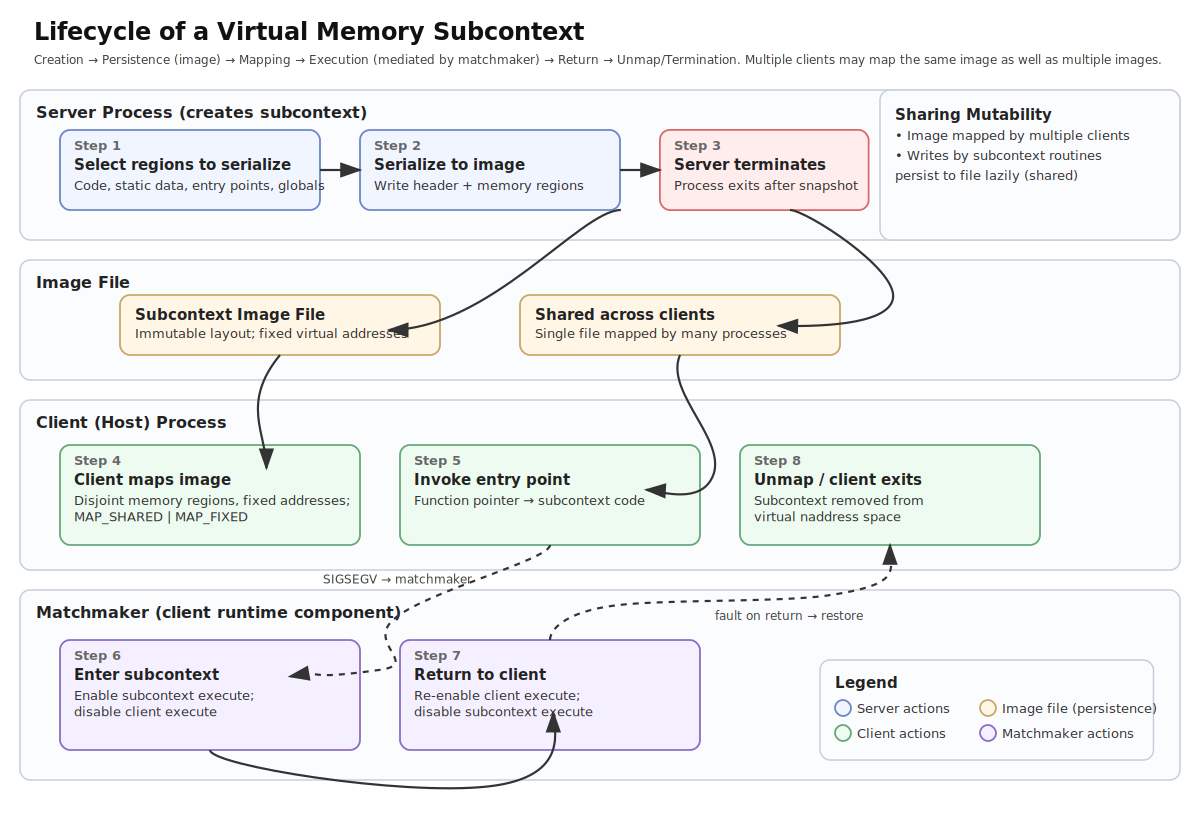
\includegraphics[width=\textwidth]{subcontext_lifecycle.png}
    \caption{The lifecycle of a subcontext.}
\end{figure}


\subsection*{Memory Topology and Placement}
\addcontentsline{toc}{subsection}{Memory Topology and Placement}
Subcontexts are mapped into the address space of a client process at fixed locations, which makes mapping impossible if overlapping mappings already exist. Once placed, subcontext pages are immobile—meaning they are fixed at their mapped addresses to preserve pointer validity and layout expectations.

We assume that modern systems offer sufficiently large and sparsely used virtual address spaces to allow this strategy to scale. The pinned placement avoids the need for complex relocation or dynamic symbol resolution.

A registry of all active subcontext mappings is maintained on the client side (specifically, within the matchmaker) to coordinate memory layout, enforce safety policies, and support runtime instrumentation.

\begin{figure}[ht]
    \centering
    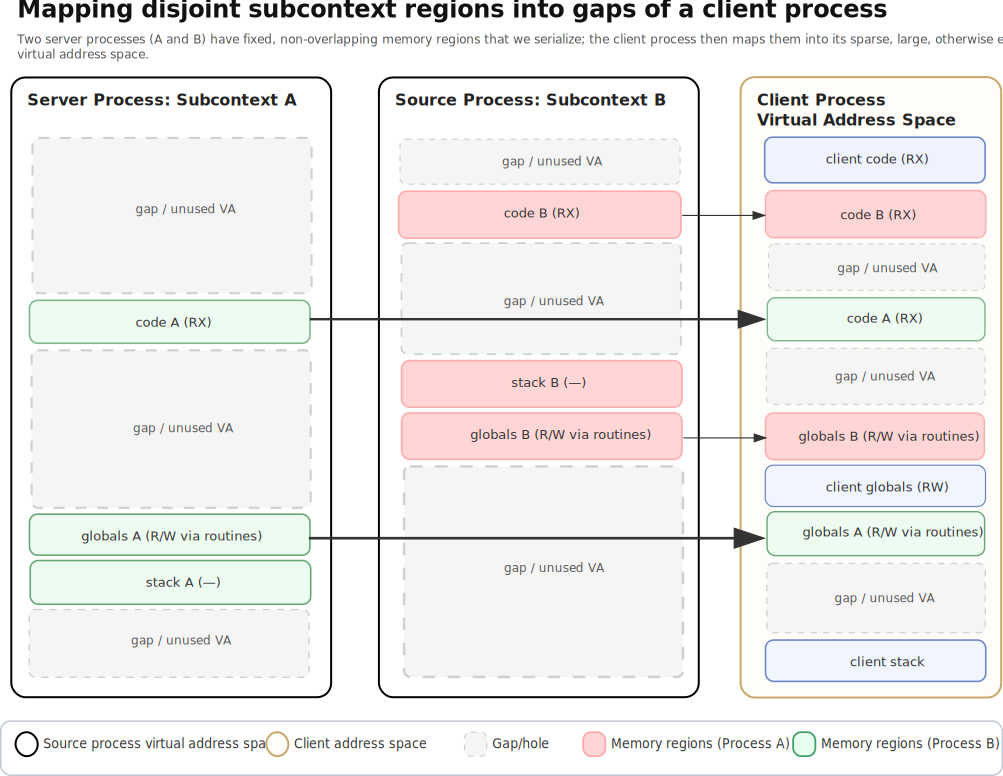
\includegraphics[width=\textwidth]{subcontexts_slotting_into_client.png}
    \caption{This is what the virtual address space of a client process looks like when it has mapped several subcontext.}
\end{figure}

\newpage
\section*{Architecture Overview}
\addcontentsline{toc}{section}{Architecture Overview}
The system is divided into three natural, primary roles: the \textbf{server-side library}, which is responsible for the creation of subcontexts; the 
\textbf{client-side library}, which maps and invokes subcontexts; and the \textbf{matchmaker}, which is part of the client library and enforces protections at runtime. This tripartite model emerged during prototyping in response to challenges around memory protection, control flow, and execution boundaries.

Initially, only the server and client roles were envisioned. The server generates image files, and the client loads and invokes them. However, ensuring memory safety required a third component: a runtime mediator that could enforce permissions during execution time and manage transitions. This mediator became the \textit{matchmaker}.

\subsection*{The Server-Side Library}
\addcontentsline{toc}{subsection}{The Server-Side Library}
The server-side library allows a process to serialize its own memory into an image file. This involves identifying relevant regions, reading their contents, and writing them into a structured binary file. Each serialized region is described in a header section that includes metadata such as the region’s starting address, size, permissions, and offset in the file. This metadata enables later reconstruction of the original memory layout during mapping by the client process, meaning that image files well-suited for reuse and distribution across processes.

\newpage
\subsubsection*{An Example Program}
The following program serializes its memory into an image file by picking up the methods provided by the server-side library.

\begin{ccode}
#include <stdio.h>
#include <stdlib.h>
#include "vm_sbc.h" // the header file for our system libraries

// the function to be serialized
void function1(int arg) {
	printf("Hello, world! arg=%d\n", arg);
}

int main(void) {
	// slot a pointer to the desired function into an array
	void (*funcs[1])(int) = { function1 };

	/* create_image_file is the library method which serializes
	 * and stores the snapshot of the memory of the process
	 */
	if (create_image_file(__FILE_NAME__, funcs, 1) != EXIT_SUCCESS) {
		fprintf(stderr, "Failed to create image file\n");
		return EXIT_FAILURE;
	}
}
\end{ccode}

\subsection*{The Client-Side Library}
\addcontentsline{toc}{subsection}{The Client-Side Library}
The client-side library supports mapping subcontext image files into memory and invoking their functionality. It uses the metadata in the image file to allocate a safe region in virtual memory, map each subcontext page with correct permissions, and link internal function pointers.

Once mapped, the client can invoke subcontext functions directly, treating the subcontext as a static, read-only module. The client is prohibited from modifying subcontext memory, and the subcontext has no access to client memory.

A global list of all mapped subcontexts is maintained by the matchmaker, which is a component of the client-side library which allows it to resolve which region of memory is active and to enforce protection boundaries dynamically.

\subsubsection*{An Example Program}
The following program maps an available image file into its memory as a subcontext via the client-side library and executes any available functions residing within the memory of the subcontext.

\begin{ccode}
#include <stdio.h>
#include <stdlib.h>
#include "vm_sbc.h" // the header file for our system libraries

int main(int argc, char **argv) {

	// check for the appropriate number of arguments
	if (argc < 2) {
		fprintf(stderr, "Usage: %s <img_file> [img_file...]\n", argv[0]);
		return EXIT_FAILURE;
	}

	/* init is a client-side library method that
	 * initializes both the matchmaker as well as 
	 * the entirety of the client-side library.
	 */
	init();

	int fds[MAX_IMG_FILES];
	size_t num_fds = 0;

	for (int i = 1; i < argc && num_fds < MAX_IMG_FILES; i++) {
		const char *img = argv[i] // the image file to map
		printf("Mapping image file: %s\n", img);

		/* map_subcontext is a client-side library method
		 * that maps the desired image file into the memory
		 * of the client process
		 */
		int fd = map_subcontext(img);
		if (fd < 0) {
			fprintf(stderr, "Failed to map %s\n", img);
			continue;
		}
		fds[num_fds++] = fd;

		int idx = 0;
		/* call_subcontext_function is a client-side
		 * library method which attempts to call a function
		 * residing in the memory of the mapped subcontext
		 */
		while (call_subcontext_function(idx, fd) == EXIT_SUCCESS) idx++;
		printf("Executed %d functions from %s\n", idx, img);

	}

	/* finalize is a client-side library method
	 * belonging to the matchmaker which disables
	 * all subcontext execute permissions and enables
	 * client execute permissions.
	 */
	finalize();
	return EXIT_SUCCESS;
}
\end{ccode}

This program begins by checking that the right number of arguments were provided by the user. The user should provide the names of image files they desire to map into the memory of the client process as subcontexts. They can provide up to \cinline{MAX_IMG_FILES} names of image files that exist.

The next step is to initialize the client-side library (which includes the matchmaker). This should always be done by user programs before attempting to utilize methods from the library. \cinline{init()} installs the segfault handler and ensures that the list of mapped subcontext and client memory regions are both zeroed out and prepared to account for any subcontexts which might presently be mapped in.

Next, the program enters a loop which maps the desired image files into its own memory (provided that they exist) as subcontexts and calls all functions available within the memory of the subcontext.

The program closes with a call to \cinline{finalize()}, which should always be called at the end of a user program, and should not be omitted. This method ensures that the matchmaker appropriately sets permissions--that all execute permissions for any mapped subcontexts are disabled and that the execute permissions for the client are enabled.

\subsection*{The Matchmaker}
\addcontentsline{toc}{subsection}{The Matchmaker}
The matchmaker is a runtime component that acts as a memory protection manager. It is part of the client-side library and ensures that when control flow enters a mapped subcontext, execution permissions are removed from the code regions of the client process and granted to those of the subcontext. When control returns to the client process, these permissions are reversed.

This toggling is implemented using page protection and signal trapping. When a client attempts to execute code in an unpermitted region, a \cinline{SIGSEGV} signal is triggered. The matchmaker intercepts the signal, inspects the instruction pointer, and adjusts page permissions accordingly before resuming execution.

This mechanism creates a well-defined entry point model: subcontext entry is only permitted at agreed-upon points, and all transitions are tightly controlled. The matchmaker enforces asymmetric visibility which means that clients know about subcontexts, but subcontexts remain unaware of the client process in which they are mapped or of other subcontexts.

We considered an alternative design where the matchmaker would itself be implemented as a subcontext, implicitly mapped into every client during initialization. However, this added unnecessary indirection. Embedding the matchmaker directly into the client library proved simpler and more robust.

% implementation details
\chapter*{IMPLEMENTATION DETAILS}
\thispagestyle{fancy}
\addcontentsline{toc}{chapter}{IMPLEMENTATION DETAILS}

\section*{Overview of Implementation Goals and Constraints}
\addcontentsline{toc}{section}{Overview of Implementation Goals and Constraints}
This prototype was implemented in C on Linux, in user-space and utilizing only user-space facilities. The language choice reflects the need for precise and low-level control over memory layout, permissions, and signal handling. In particular, C allows for the direct use of system calls like \cinline{mmap}, \cinline{mprotect}, and \cinline{sigaction}, which are central to managing memory and handling page faults at a very low-level in user space.

Our prototype was developed under several constraints, the most important of which being that we made no kernel modifications. That is, our prototype exists only in user-space and utilizes only user-space facilities. All protections and transitions must be enforced at the user level. Our implementation targets Linux specifically, although future work may include portability to other UNIX-like systems. Given time constraints, we chose to adopt a minimal design that still acted as a concrete proof-of-concept. In future, we would like to extend this design to more completely and thoroughly embody the concept at the heart of this prototype.

\newpage
\section*{Codebase and File Structure}
\addcontentsline{toc}{section}{Codebase and File Structure}
The codebase is split across four files:
\begin{itemize}
    \item \cinline{sbc_server.c}: Handles memory serialization logic as well as the creation of image files.
    \item \cinline{sbc_client.c}: Implements memory mapping and function invocation for subcontexts.
    \item \cinline{sbc_mm.c}: The matchmaker implementation, which handles memory protection and signal handling logic.
    \item \cinline{vm_sbc.h}: A header file. Contains shared data structures, constants, and declarations across modules.
\end{itemize}

This modular structure facilitates reuse and delimits the conceptual boundaries outlined in the previous section. Common types, constraints, and function stubs live in the header, while each source file maintains responsibility for a specific phase of the subcontext lifecycle.

\section*{Server Implementation}
\addcontentsline{toc}{section}{Server Implementation}
The server is responsible for identifying memory regions to serialize as well as creating an image file that represents a process frozen at a given moment in time. It begins by inspecting \cinline{/proc/self/maps} to enumerate all memory regions. These regions are then parsed and filtered to exclude dynamic heap and stack segments, as well as any shared libraries or memory-mapped I/O regions. We chose to exclude these regions because they were unnecessary for function invocation from within a client process.

Each memory segment to be serialized in the image file is represented by an `Entry` struct, which stores its virtual address range, permissions, and offset into the file. These structures are organized into an array, which becomes the header for the image file.

This header includes:
\begin{itemize}
    \item The number of memory regions present in or copied from the target process
    \item Virtual address ranges for each regions
    \item Permissions (read/write/execute)
    \item Offset values indicating where in the file each region's contents begin
    \item An array of pointers to the functions defined by the process contained within the image file
\end{itemize}

After writing the header, the contents of each region are copied bit-for-bit using \cinline{memcpy}. Once the image is complete, the server exits. Its memory is now captured entirely in a reusable binary format, ready to be mapped by any client.

\section*{Client Implementation}
\addcontentsline{toc}{section}{Client Implementation}
The client reads an image file, maps its memory regions into disjoint parts of its own virtual address space, and invokes predefined functions defined within the subcontext.

The client begins by opening the image file and parsing the header. It ensures that the fixed virtual address ranges of the subcontext do not overlap with its own occupied virtual address ranges. If such an overlap is found for any given region present in the image file, the program terminates with an error. If no overlap is found, information about the subcontext is stored into a global data structure.

Next, each segment is mapped with all permissions (i.e., \cinline{PROT_READ}, \cinline{PROT_WRITE}, and \cinline{PROT_EXEC}) to be modified to appropriate permissions based on the original serialized state by the matchmaker later, as we intended to use \cinline{mprotect} to turn off permissions already granted rather than to turn on permissions previously denied. These mappings utilize the \cinline{MAP_SHARED | MAP_FIXED} flags to ensure that the memory of a given mapped subcontext is shared across all of the client processes that map it and that the mapping of the subcontext's memory regions occurs in the locations previously specified.

The client maintains an internal linked list of active subcontexts using a \cinline{MappedSubcontext} struct, which tracks base address, size, entry points, and usage flags, among other things. Usage of this data structure allows efficient lookup and execution routing.

Function calls into subcontext memory are performed using predefined entry point offsets. These are cast to known function signatures using function pointers. All invocations are mediated by the matchmaker to ensure that execute permissions are toggled appropriately, directly before and after each call.

\section*{Matchmaker and Safety Enforcement}
\addcontentsline{toc}{section}{Matchmaker and Safety Enforcement}
The matchmaker acts at runtime and is embedded in the client library. Its primary role is to enforce memory execution boundaries between client code and subcontext code. This is achieved by registering a custom \cinline{SIGSEGV} handler using \cinline{sigaction}and dynamically toggling execute permissions using \cinline{mprotect}.

When a client invokes a function which resides in a subcontext, the matchmaker first disables all executable pages in the client’s address space and enables pages belonging to the subcontext. Excluded pages include those required for minimal runtime support, as well as those containing \cinline{[vvar]} and \cinline{[vdso]}, for if the pages contained within these regions are disabled, an \cinline{ENOMEM} error occurs.

Once execution returns to client code, a page fault is triggered on an unmapped or non-executable client address. This transfers control to the \cinline{SIGSEGV} handler, which recognizes the transition and reverses the permission mappings accordingly. If the address does not belong to any mapped subcontext, the custom handler cannot resolve the fault, so the \cinline{SIGSEGV} signal is re-raised with the default, so that the process does not endlessly loop in the handler.

All active subcontexts are registered in a global table that stores their address range, state, and associated permissions. The matchmaker consults this table to determine which pages to re-enable or disable.

\section*{System Interfaces Used}
\addcontentsline{toc}{section}{System Interfaces Used}
We rely on several methods belonging to the Standard C Library (\cinline{libc}) API:
\begin{itemize}
    \item \cinline{mmap}: For allocating memory and mapping file-backed regions into virtual address spaces.
    \item \cinline{mprotect}: For toggling page permissions.
    \item \cinline{sigaction}: For installing a custom signal handler.
    \item \cinline{memcpy}: For copying memory into files.
\end{itemize}

Our implementation also depends on the kernel feature \cinline{/proc/self/maps}, the use of which allows us to discover the memory layout of the current process. These interfaces allow us to build the system entirely in user space, at the cost of some safety guarantees that presence in the kernel would alleviate.

\section*{User Experience}
\addcontentsline{toc}{section}{User Experience}
From the perspective of a user or developer, working with subcontexts of virtual memory is both similar to and different from conventional shared library usage. In the current implementation, developers must include the header file \cinline{vm_sbc.h} to gain access to the virtual memory subcontext API in addition to compiling their programs with the server-side library (\cinline{libsbcserver.a}) or the client-side library (\cinline{libsbcclient.a}). In future, we hope to eliminate this dependency on the shared library format in favor of the static library format.

In terms of use, the API is intuitive and intentionally minimal. Creating a subcontext involves a single call to a function which serializes designated memory regions. Mapping a subcontext from an image file is equally straightforward. All details of low-level address space management are abstracted away. This means that developers need not consider virtual offsets or page alignment problems, as these are handled internally by the system.

Debugging errors related to subcontext use is slightly less straightforward. Error handling is minimal and only follows standard C conventions, providing features such as minimal return codes to simplify debugging. Future development should focus at least in part on debugging tools.

Utilizing subcontexts feels similar to normal function calls from the developer's perspective, with only one added layer of abstraction between the developer and the desired function. Latency in function calls, matchmaker mediation, and the mapping and unmapping of subcontexts from within the virtual address space of a client process is not something our implementation explored at any reasonable depth.

Overall, the provided libraries integrate cleanly with any existing code and require little to no refactoring, meaning that developers can focus on the logic they want to share, while the system handles enforcement of safety guarantees internally.


\section*{Summary and Future Implementation Directions}
This prototype demonstrates a proof-of-concept of virtual memory subcontexts, built using only user-space tools. We’ve implemented serialization, mapping, and execution transitions between isolated code regions with no kernel support. While limited, the prototype validates the core concept while remaining extensible.

% REMOVE THIS SECTION? COVERED EXTENSIVELY IN OTHER SECTION...
To this end, future implementation efforts may include:
\begin{itemize}
    \item Moving matchmaker logic into the kernel or a privileged user-space daemon.
    \item Ensuring thread-safeness, and thus support for multi-threaded clients.
    \item Adding support for debugging and tracing.
    \item Implementing a richer image format with compression.
    \item Exploring static linking or ELF post-processing.
\end{itemize}

While our implementation is only a first approximation, it demonstrates the feasibility of the system and reveals novel abstractions whose applications impact code reusability and the implicit protections such reusability provides.

% discussion
\chapter*{DISCUSSION}
\thispagestyle{fancy}
\addcontentsline{toc}{chapter}{DISCUSSION}

Subcontexts of virtual memory aim to displace the reliance on shared libraries by enabling modular, reusable code to coexist with strict memory isolation. The motivation is primarily architectural: to allow trusted logic to be embedded directly within a client’s virtual address space, without sacrificing protection guarantees. Conventional shared libraries trust their host programs and therefore cannot be protected from them, creating the need for protection to be enforced by some kind of barrier--normally syscalls (for services provided by the kernel) or some flavor of kernel mediation (for user-mode services). Subcontexts, on the other hand, allow code invocation to occur across clearly defined memory boundaries, with minimal performance penalty. In this sense, subcontexts seek to both \textit{replace} and \textit{improve upon} traditional dynamic linking by disallowing client process modification of subcontext memory except through well-defined entry points.

\section*{Architecture and Design Insights}
\addcontentsline{toc}{section}{Architecture and Design Insights}
The division into \textbf{server}, \textbf{client}, and \textbf{matchmaker} components emerged as a natural architectural response to the problem at hand. The server-side library handles serialization, the client-side library handles mapping and utilization, and the matchmaker mediates interaction between them. And while the server-client split was intuitive, the matchmaker evolved through trial and error. It was originally conceptualized as a subcontext in and of itself: it was to be an image file that client processes would implicitly and automatically map into their virtual memory as they picked up the client-side library. It was later restructured as a lightweight runtime component embedded within the client library. This design choice unnecessary indirection while still enforcing execution protections.

These protections are implemented using a \cinline{SIGSEGV} handler installed by the matchmaker. When a client process attempts to execute code in a subcontext region without the appropriate permissions, the fault is intercepted, and permissions are granted or revoked in a well-defined manner. This seemed the most straightforward way to mediate the interaction between client processes and their mapped subcontexts.

\section*{Strengths of the Subcontext Model}
\addcontentsline{toc}{section}{Strengths of the Subcontext Model}
The most evident strength of the subcontext model is its modularity. Subcontexts are packaged in self-contained image files that can be picked up and mapped by any client process. This facilitates reuse free of recompilation or relinking. Multiple subcontexts can be mapped into a single client process, and the same subcontext can be simultaneously mapped by many clients, all without additional synchronization overhead. This capability for parallel mapping gives subcontexts a performance advantage over more traditional modularity mechanisms.

Subcontexts also improve performance by avoiding overhead typically associated with  calls made between processes. Because they are invoked directly from within the address space of the client process without syscalls or context switches, function calls into a mapped subcontext are extremely lightweight.

Another key strength is trust isolation. Clients cannot modify subcontext memory except through well-defined entry points and behavior specified only in subcontext routines. That is, even if a subcontext exposes a writable data structure (e.g., a global counter), it must do so deliberately, and always through routines defined within the subcontext itself. This controlled exposure makes the model inherently safer than shared libraries, which immediately and implicitly share the protection boundary of the host.

Finally, our design abstracts away implementation details, making it agnostic of both language and system. While our prototype targets Linux and is written in C, its core design principles could be adapted to other systems with similar virtual memory models, or to other languages that allow for low-level memory management.

\section*{Limitations of the Current Prototype}
\addcontentsline{toc}{section}{Limitations of the Current Prototype}
Despite these strengths, there are several limitations of our implementation our assumptions upon which it depends.

\subsection*{1. Thread-Agnosticism}
\addcontentsline{toc}{subsection}{Thread-Agnosticism}
Our prototype is agnostic towards thread-management and for this reason does not support multi-threaded client processes, although it must be noted that a mapped subcontext is "shared" (essentially multi-threaded) among the client processes which map it. This may become problematic in environments where client processes expect concurrent behavior or where the routines of mapped subcontext may themselves spawn threads. This also means that uncoordinated access to a shared mapped subcontext introduces race conditions unless handled explicitly. For example, support for \cinline{pthread}s is currently broken under this model.

\subsection*{2. Fixed Address Mapping and Memory Fragmentation}
\addcontentsline{toc}{subsection}{Fixed Address Mapping and Memory Fragmentation}
Subcontexts are mapped from their image files into fixed, pre-defined memory ranges. If a client process already occupies any of these regions, mapping fails entirely. This makes the system brittle in the face of address space fragmentation and severely limits compatibility with large, dynamic applications. The current design assumes that client processes have large swaths of unused virtual memory available, which is not always a safe assumption to make.

\subsection*{Image Format and Entry Point Rigidity}
\addcontentsline{toc}{subsection}{Image Format and Entry Point Rigidity}
Our image format is deliberately minimal. It performs no compression or address relocation and stores only raw segments. Client processes must know entry point offsets ahead of time and cast raw function pointers into callable code. This limits portability, makes introspection difficult, and introduces potential safety hazards (e.g., if function boundaries are misaligned or corrupted).

Additionally, because subcontexts are fixed-size post-serialization, dynamic memory allocation within them is potentially unsafe. Any attempt to allocate memory beyond the serialized footprint may result in errors or undefined behavior.

\subsection*{4. Dynamic Linking Constraints}
\addcontentsline{toc}{subsection}{Dynamic Linking Constraints}
Currently, both the client and server libraries are `.so` (shared object) files. This choice restricts how symbols are resolved and creates some fragility in the linking process. In earlier iterations, we encountered linker issues where symbols from the serialized program failed to resolve unless they had been invoked \textit{before} serialization. Moving the serialization logic into a separate translation unit alleviated this issue, but highlighted the complex interplay between static linkage, dynamic resolution, and runtime behavior.

\subsection*{5. User-Space Enforcement Only}
\addcontentsline{toc}{subsection}{User-Space Enforcement Only}
Perhaps the most consequential limitation of our implementation is the prototype’s user-space confinement. Without kernel-level enforcement, we rely entirely on user-level page permissions and fault handlers. A malicious client process could conceivably bypass the matchmaker or tamper with mapped image pages. Without kernel-mediated memory isolation, the current security guarantees are weaker than would otherwise be desired.

\section*{Implementation Challenges and Surprises}
\addcontentsline{toc}{section}{Implementation Challenges and Surprises}
Several implementation surprises arose over the course of development. Most notably, linker behavior proved non-deterministic when serialization was performed within the same translation unit as the main program logic. Symbols belonging to uninvoked functions were pruned or left unresolved after serialization, leading to broken mappings. This issue disappeared when serialization logic was split into a separate file. This demonstrated to us the opaque nature of modern linkers as they relate to unused symbols.

Another surprise was how well the segmentation fault handler approach worked to enforce control flow transitions. Though crude in some ways, it provided a clear and effective method for managing execution privileges without kernel support or binary rewriting.

% open questions and future work
\chapter*{FUTURE WORK AND OPEN QUESTIONS}
\thispagestyle{fancy}
\addcontentsline{toc}{chapter}{FUTURE WORK AND OPEN QUESTIONS}

The development of our prototype for virtual memory subcontexts left in its wake several open questions and exposed avenues for future exploration. Some directions were constrained by time, while others only became clear through the process of implementation. This section outlines possible technical extensions and one especially unresolved implementation-level puzzle that we encountered during development.

\section*{1. Kernel Integration and Hardware Enforcement}
\addcontentsline{toc}{section}{Kernel Integration and Hardware Enforcement}
Currently, our prototype resides entirely in user space. As a result, memory protection depends exclusively on user-level APIs such as \cinline{mprotect}, which are inherently brittle, reactive, and subject to user-space interference. A kernel-level implementation could offer more robust guarantees. By handling subcontext mapping at the kernel level and managing access permissions directly through the page table, we could avoid many of the coordination problems that plague user-space enforcement and boost performance with a more elegant design.

Future work could include the development of a minimal kernel module or the use of existing kernel APIs to intercept and manage page faults during subcontext entry. Ultimately, we imagine a future in which subcontexts become a first-class kernel primitive, similar to memory namespaces or shared memory segments, with native support from the operating system and CPU.

\section*{2. Support for Multi-Threading}
\addcontentsline{toc}{section}{Support for Multi-Threading}
Our current implementation is thread-agnostic and assumes a single-threaded execution model. We made no attempt to address concurrency, synchronization, or thread-specific subcontext transitions. However, supporting multi-threaded client processes poses a number of complications. Page permissions in Linux are enforced per-process, not per-thread. As a result, if one thread attempts to enter a subcontext and toggles execute permissions, other threads might simultaneously lose access to their expected code regions.

One possible solution involves thread-local subcontext state, with the matchmaker coordinating transitions on a per-thread basis. However, this may require complex cooperation between signal handlers and thread schedulers. Alternatively, we must ask whether subcontexts are fundamentally serial in nature (i.e., whether only one thread at a time should ever enter a given subcontext) and if so, whether concurrency should even be a target for future development.

\section*{3. Enhanced Image Compression}
\addcontentsline{toc}{section}{Enhanced Image Compression}
The current image format is deliberately simple. It captures raw memory segments without any form of compression or optimization. Clients must know function entry offsets in advance and cast function pointers manually. While this simplicity aids debugging and transparency, it misses opportunities for compression, improved safety, and more expressive memory modeling.

Future work could include support for sparse memory layouts, compression of zeroed pages, and exclusion of redundant metadata. These improvements would reduce image size and improve memory utilization. Additionally, the current image files are fixed-size post-serialization. If a subcontext allocates dynamic memory beyond its pre-allocated region, it risks accessing unmapped or unallocated pages—potentially causing segmentation faults or undefined behavior. Future versions could implement flexible image layouts or embedded allocators to support controlled post-mortem heap growth.

\section*{4. ELF Segment and Linking Behavior}
\addcontentsline{toc}{section}{ELF Segment and Linking Behavior}
Although our server and client logic currently reside in shared libraries (\cinline{.so} files), our broader goal is to replace or improve upon the shared library model. This raises the question: can we entirely avoid dynamic linking? Future work may involve constructing subcontext binaries as static ELF executables, with embedded serialization metadata, so that clients can load and execute them without depending on runtime-shared objects.

Such an approach would likely require low-level manipulation of ELF headers and custom linking logic. While this would increase binary size and complexity, it would also offer greater control over symbol resolution and eliminate runtime dependencies—making subcontexts more portable, robust, and self-contained.

\section*{5. Developer Tools and Higher-Level Bindings}
\addcontentsline{toc}{section}{Developer Tools and Higher-Level Bindings}
Although our prototype demonstrates the basic feasibility of subcontexts, its interface is minimal and assumes a C-style, manual low-level memory management model. In the future, we hope to extend subcontext capabilities to higher-level programming environments through transpilation tools. These could abstract away low-level memory operations and provide safer, language-integrated interfaces for invoking subcontext functionality.

In addition, tooling for debugging and development remains primitive. Visualizing image layout, tracking subcontext transitions, and inspecting memory usage would greatly aid both users and developers. Future work could include interactive introspection tools, symbolic subcontext debuggers, and static analysis pipelines for preparing programs for serialization.

\section*{Open Technical Questions}
\addcontentsline{toc}{section}{Open Technical Questions}
One especially persistent technical issue emerged during implementation. Initially, we embedded the serialization logic within the same binary as the server program. After serialization, we found that symbols for functions that had not yet been invoked at runtime failed to resolve when invoked after mapping. In contrast, any function called prior to serialization had its symbol correctly resolved and preserved.

We attempted to resolve this using various linker and loader flags but had no success. The only consistent workaround was to ensure that all functions we wished to serialize were invoked at least once prior to serialization.

Surprisingly, this issue disappeared when we moved the serialization logic into a separate library. When the server merely linked against this external serialization module, the resulting image preserved symbols for all linked functions, even if they were never called.

We suspect this has to do with how linkers and dynamic loaders resolve and record symbols based on usage during static linking and lazy resolution during runtime. However, the exact cause remains unclear. Future work could involve a deeper investigation into the internals of the dynamic linker and symbol resolution mechanisms to determine why embedding serialization logic inside the server binary suppresses unresolved symbols.

% conclusion
\chapter*{CONCLUSION}
\thispagestyle{fancy}
\addcontentsline{toc}{chapter}{CONCLUSION}
Shared libraries, while ubiquitous, inherently adopt the protection boundaries of the processes into which they are linked. This presents a longstanding architectural limitation: once a trusted library is dynamically linked into an untrusted process, it itself becomes untrusted, and is thus exposed to potential misuse or corruption. This problem is particularly acute in low-level languages like C, where memory safety cannot be assumed. Our work addresses this issue by introducing subcontexts of virtual memory, a novel abstraction that seeks to preserve the modularity of shared libraries while restoring their original protection boundary.

In this thesis, we have designed, implemented, and evaluated a prototype system that demonstrates the conceptual and practical feasibility of virtual memory subcontexts. Essentially, a subcontext is a frozen snapshot of a process--a serialized and invokable swath of (possibly discontiguous) memory. Subcontexts can be mapped into a client process's virtual address space and safely invoked, without requiring dynamic linking or kernel-level privilege transitions. The design relies on a tripartite architecture consisting of a server-side library (to create subcontexts), a client-side library (to map and invoke them), and a matchmaker (part of the client-side library, responsible for managing execution-time memory protections). Together, these components enable a new memory-sharing paradigm that is safe, lightweight, and modular.

We demonstrated that it is indeed possible to embed trusted logic inside an untrusted process without relinquishing protection guarantees by compromising memory isolation. However, our work also makes clear the limitations and open challenges that remain. The current prototype is single-threaded, limited in its image file format, and still relies on shared libraries for implementation. Additionally, the client-server interface is coarse, and our design assumes generous availability of unused virtual memory in modern processes, an assumption that may not hold in more constrained environments. Perhaps most critically, development of our prototype revealed a problems with the dynamic linker in the presence of aggressive memory remapping, which poses challenges for long-term subcontext stability and integration into real-world applications.

Despite these limitations, we believe our results are both encouraging and instructive. They offer a new way to think about modularity and trust in systems design that prioritizes memory safety and control over traditional linking convenience. Subcontexts may not replace shared libraries outright, but they offer a complementary model that could be especially valuable in high-assurance systems, sandboxing, or modular runtime environments.

This project was born from a vague, almost architectural impulse—an intuition about the nature of modularity, trust, and memory. Through iterative implementation and experimentation, we shaped that intuition into a functioning system. In doing so, we not only built a working prototype, but also clarified the conceptual space that subcontexts inhabit: somewhere between a library and a process.

Future work will explore integration with the kernel, support for multi-threading, more sophisticated file formats, and perhaps even hardware-enforced variants of subcontexts. We envision a world in which processes can safely compose functionality at runtime by embedding trusted modules that retain their own protection boundaries, even when embedded in the memory of other untrusted modules.

Subcontexts challenge the traditional boundaries of trust and memory in operating systems. They do not replace our existing abstractions. They augment them by offering a new lens through which we might rethink the architecture of shared functionality.


% link to codebase
\chapter*{A LINK TO OUR CODEBASE}
\thispagestyle{fancy}
\addcontentsline{toc}{chapter}{A LINK TO OUR CODEBASE}

The codebase for the implementation of the prototype for virtual memory subcontexts is contained within this \href{https://github.com/riddlework/vm_subcontexts}{repository}\footnote{\href{https://github.com/riddlework/vm_subcontexts}{https://github.com/riddlework/vm\_subcontexts}}, which is hosted on Github. It contains all the source and testing code for our prototype, as well as the LaTeX source code for this thesis, which was adapted from the University of Arizona's standard graduate dissertation template.



\end{document}